\documentclass[twoside]{book}

% Packages required by doxygen
\usepackage{fixltx2e}
\usepackage{calc}
\usepackage{doxygen}
\usepackage[export]{adjustbox} % also loads graphicx
\usepackage{graphicx}
\usepackage[utf8]{inputenc}
\usepackage{makeidx}
\usepackage{multicol}
\usepackage{multirow}
\PassOptionsToPackage{warn}{textcomp}
\usepackage{textcomp}
\usepackage[nointegrals]{wasysym}
\usepackage[table]{xcolor}

% Font selection
\usepackage[T1]{fontenc}
\usepackage[scaled=.90]{helvet}
\usepackage{courier}
\usepackage{amssymb}
\usepackage{sectsty}
\renewcommand{\familydefault}{\sfdefault}
\allsectionsfont{%
  \fontseries{bc}\selectfont%
  \color{darkgray}%
}
\renewcommand{\DoxyLabelFont}{%
  \fontseries{bc}\selectfont%
  \color{darkgray}%
}
\newcommand{\+}{\discretionary{\mbox{\scriptsize$\hookleftarrow$}}{}{}}

% Page & text layout
\usepackage{geometry}
\geometry{%
  a4paper,%
  top=2.5cm,%
  bottom=2.5cm,%
  left=2.5cm,%
  right=2.5cm%
}
\tolerance=750
\hfuzz=15pt
\hbadness=750
\setlength{\emergencystretch}{15pt}
\setlength{\parindent}{0cm}
\setlength{\parskip}{3ex plus 2ex minus 2ex}
\makeatletter
\renewcommand{\paragraph}{%
  \@startsection{paragraph}{4}{0ex}{-1.0ex}{1.0ex}{%
    \normalfont\normalsize\bfseries\SS@parafont%
  }%
}
\renewcommand{\subparagraph}{%
  \@startsection{subparagraph}{5}{0ex}{-1.0ex}{1.0ex}{%
    \normalfont\normalsize\bfseries\SS@subparafont%
  }%
}
\makeatother

% Headers & footers
\usepackage{fancyhdr}
\pagestyle{fancyplain}
\fancyhead[LE]{\fancyplain{}{\bfseries\thepage}}
\fancyhead[CE]{\fancyplain{}{}}
\fancyhead[RE]{\fancyplain{}{\bfseries\leftmark}}
\fancyhead[LO]{\fancyplain{}{\bfseries\rightmark}}
\fancyhead[CO]{\fancyplain{}{}}
\fancyhead[RO]{\fancyplain{}{\bfseries\thepage}}
\fancyfoot[LE]{\fancyplain{}{}}
\fancyfoot[CE]{\fancyplain{}{}}
\fancyfoot[RE]{\fancyplain{}{\bfseries\scriptsize Generated by Doxygen }}
\fancyfoot[LO]{\fancyplain{}{\bfseries\scriptsize Generated by Doxygen }}
\fancyfoot[CO]{\fancyplain{}{}}
\fancyfoot[RO]{\fancyplain{}{}}
\renewcommand{\footrulewidth}{0.4pt}
\renewcommand{\chaptermark}[1]{%
  \markboth{#1}{}%
}
\renewcommand{\sectionmark}[1]{%
  \markright{\thesection\ #1}%
}

% Indices & bibliography
\usepackage{natbib}
\usepackage[titles]{tocloft}
\setcounter{tocdepth}{3}
\setcounter{secnumdepth}{5}
\makeindex

% Hyperlinks (required, but should be loaded last)
\usepackage{ifpdf}
\ifpdf
  \usepackage[pdftex,pagebackref=true]{hyperref}
\else
  \usepackage[ps2pdf,pagebackref=true]{hyperref}
\fi
\hypersetup{%
  colorlinks=true,%
  linkcolor=blue,%
  citecolor=blue,%
  unicode%
}

% Custom commands
\newcommand{\clearemptydoublepage}{%
  \newpage{\pagestyle{empty}\cleardoublepage}%
}

\usepackage{caption}
\captionsetup{labelsep=space,justification=centering,font={bf},singlelinecheck=off,skip=4pt,position=top}

%===== C O N T E N T S =====

\begin{document}

% Titlepage & ToC
\hypersetup{pageanchor=false,
             bookmarksnumbered=true,
             pdfencoding=unicode
            }
\pagenumbering{roman}
\begin{titlepage}
\vspace*{7cm}
\begin{center}%
{\Large Group 7 Homework }\\
\vspace*{1cm}
{\large Generated by Doxygen 1.8.11}\\
\end{center}
\end{titlepage}
\clearemptydoublepage
\tableofcontents
\clearemptydoublepage
\pagenumbering{arabic}
\hypersetup{pageanchor=true}

%--- Begin generated contents ---
\chapter{Namespace Index}
\section{Packages}
Here are the packages with brief descriptions (if available)\+:\begin{DoxyCompactList}
\item\contentsline{section}{\hyperlink{namespacecom}{com} }{\pageref{namespacecom}}{}
\item\contentsline{section}{\hyperlink{namespacecom_1_1homework}{com.\+homework} }{\pageref{namespacecom_1_1homework}}{}
\item\contentsline{section}{\hyperlink{namespacecom_1_1homework_1_1aydin}{com.\+homework.\+aydin} }{\pageref{namespacecom_1_1homework_1_1aydin}}{}
\item\contentsline{section}{\hyperlink{namespacecom_1_1homework_1_1denizalp}{com.\+homework.\+denizalp} }{\pageref{namespacecom_1_1homework_1_1denizalp}}{}
\item\contentsline{section}{\hyperlink{namespacecom_1_1homework_1_1home}{com.\+homework.\+home} }{\pageref{namespacecom_1_1homework_1_1home}}{}
\item\contentsline{section}{\hyperlink{namespacecom_1_1homework_1_1kubra}{com.\+homework.\+kubra} }{\pageref{namespacecom_1_1homework_1_1kubra}}{}
\item\contentsline{section}{\hyperlink{namespacecom_1_1homework_1_1necil}{com.\+homework.\+necil} }{\pageref{namespacecom_1_1homework_1_1necil}}{}
\item\contentsline{section}{\hyperlink{namespacecom_1_1homework_1_1salih}{com.\+homework.\+salih} }{\pageref{namespacecom_1_1homework_1_1salih}}{}
\item\contentsline{section}{\hyperlink{namespacecom_1_1homework_1_1yigit}{com.\+homework.\+yigit} }{\pageref{namespacecom_1_1homework_1_1yigit}}{}
\item\contentsline{section}{\hyperlink{namespacecom_1_1homework_1_1yunus}{com.\+homework.\+yunus} }{\pageref{namespacecom_1_1homework_1_1yunus}}{}
\end{DoxyCompactList}

\chapter{Hierarchical Index}
\section{Class Hierarchy}
This inheritance list is sorted roughly, but not completely, alphabetically\+:\begin{DoxyCompactList}
\item \contentsline{section}{com.\+homework.\+yunus.\+Db\+Yunus}{\pageref{classcom_1_1homework_1_1yunus_1_1_db_yunus}}{}
\item Http\+Servlet\begin{DoxyCompactList}
\item \contentsline{section}{com.\+homework.\+home.\+Home}{\pageref{classcom_1_1homework_1_1home_1_1_home}}{}
\item \contentsline{section}{com.\+homework.\+yunus.\+Yunus}{\pageref{classcom_1_1homework_1_1yunus_1_1_yunus}}{}
\end{DoxyCompactList}
\end{DoxyCompactList}

\chapter{Class Index}
\section{Class List}
Here are the classes, structs, unions and interfaces with brief descriptions\+:\begin{DoxyCompactList}
\item\contentsline{section}{\hyperlink{classcom_1_1homework_1_1aydin_1_1_aydin}{com.\+homework.\+aydin.\+Aydin} }{\pageref{classcom_1_1homework_1_1aydin_1_1_aydin}}{}
\item\contentsline{section}{\hyperlink{classcom_1_1homework_1_1aydin_1_1_d_b_aydin}{com.\+homework.\+aydin.\+D\+B\+Aydin} }{\pageref{classcom_1_1homework_1_1aydin_1_1_d_b_aydin}}{}
\item\contentsline{section}{\hyperlink{classcom_1_1homework_1_1denizalp_1_1_db_denizalp}{com.\+homework.\+denizalp.\+Db\+Denizalp} }{\pageref{classcom_1_1homework_1_1denizalp_1_1_db_denizalp}}{}
\item\contentsline{section}{\hyperlink{classcom_1_1homework_1_1yunus_1_1_db_yunus}{com.\+homework.\+yunus.\+Db\+Yunus} }{\pageref{classcom_1_1homework_1_1yunus_1_1_db_yunus}}{}
\item\contentsline{section}{\hyperlink{classcom_1_1homework_1_1denizalp_1_1_denizalp}{com.\+homework.\+denizalp.\+Denizalp} }{\pageref{classcom_1_1homework_1_1denizalp_1_1_denizalp}}{}
\item\contentsline{section}{\hyperlink{classcom_1_1homework_1_1home_1_1_home}{com.\+homework.\+home.\+Home} }{\pageref{classcom_1_1homework_1_1home_1_1_home}}{}
\item\contentsline{section}{\hyperlink{classcom_1_1homework_1_1kubra_1_1_kubra}{com.\+homework.\+kubra.\+Kubra} }{\pageref{classcom_1_1homework_1_1kubra_1_1_kubra}}{}
\item\contentsline{section}{\hyperlink{classcom_1_1homework_1_1aydin_1_1_model_aydin}{com.\+homework.\+aydin.\+Model\+Aydin} }{\pageref{classcom_1_1homework_1_1aydin_1_1_model_aydin}}{}
\item\contentsline{section}{\hyperlink{classcom_1_1homework_1_1yunus_1_1_model_yunus}{com.\+homework.\+yunus.\+Model\+Yunus} }{\pageref{classcom_1_1homework_1_1yunus_1_1_model_yunus}}{}
\item\contentsline{section}{\hyperlink{classcom_1_1homework_1_1necil_1_1_necil}{com.\+homework.\+necil.\+Necil} }{\pageref{classcom_1_1homework_1_1necil_1_1_necil}}{}
\item\contentsline{section}{\hyperlink{classcom_1_1homework_1_1salih_1_1_salih}{com.\+homework.\+salih.\+Salih} }{\pageref{classcom_1_1homework_1_1salih_1_1_salih}}{}
\item\contentsline{section}{\hyperlink{classcom_1_1homework_1_1aydin_1_1_sparql_aydin}{com.\+homework.\+aydin.\+Sparql\+Aydin} }{\pageref{classcom_1_1homework_1_1aydin_1_1_sparql_aydin}}{}
\item\contentsline{section}{\hyperlink{classcom_1_1homework_1_1yunus_1_1_sparql_yunus}{com.\+homework.\+yunus.\+Sparql\+Yunus} }{\pageref{classcom_1_1homework_1_1yunus_1_1_sparql_yunus}}{}
\item\contentsline{section}{\hyperlink{classcom_1_1homework_1_1yigit_1_1_yigit}{com.\+homework.\+yigit.\+Yigit} }{\pageref{classcom_1_1homework_1_1yigit_1_1_yigit}}{}
\item\contentsline{section}{\hyperlink{classcom_1_1homework_1_1yunus_1_1_yunus}{com.\+homework.\+yunus.\+Yunus} }{\pageref{classcom_1_1homework_1_1yunus_1_1_yunus}}{}
\end{DoxyCompactList}

\chapter{File Index}
\section{File List}
Here is a list of all files with brief descriptions\+:\begin{DoxyCompactList}
\item\contentsline{section}{src/com/homework/aydin/\hyperlink{_aydin_8java}{Aydin.\+java} }{\pageref{_aydin_8java}}{}
\item\contentsline{section}{src/com/homework/aydin/\hyperlink{_d_b_aydin_8java}{D\+B\+Aydin.\+java} }{\pageref{_d_b_aydin_8java}}{}
\item\contentsline{section}{src/com/homework/aydin/\hyperlink{_model_aydin_8java}{Model\+Aydin.\+java} }{\pageref{_model_aydin_8java}}{}
\item\contentsline{section}{src/com/homework/aydin/\hyperlink{_sparql_aydin_8java}{Sparql\+Aydin.\+java} }{\pageref{_sparql_aydin_8java}}{}
\item\contentsline{section}{src/com/homework/denizalp/\hyperlink{_db_denizalp_8java}{Db\+Denizalp.\+java} }{\pageref{_db_denizalp_8java}}{}
\item\contentsline{section}{src/com/homework/denizalp/\hyperlink{_denizalp_8java}{Denizalp.\+java} }{\pageref{_denizalp_8java}}{}
\item\contentsline{section}{src/com/homework/home/\hyperlink{_home_8java}{Home.\+java} }{\pageref{_home_8java}}{}
\item\contentsline{section}{src/com/homework/kubra/\hyperlink{_kubra_8java}{Kubra.\+java} }{\pageref{_kubra_8java}}{}
\item\contentsline{section}{src/com/homework/necil/\hyperlink{_necil_8java}{Necil.\+java} }{\pageref{_necil_8java}}{}
\item\contentsline{section}{src/com/homework/salih/\hyperlink{_salih_8java}{Salih.\+java} }{\pageref{_salih_8java}}{}
\item\contentsline{section}{src/com/homework/yigit/\hyperlink{_yigit_8java}{Yigit.\+java} }{\pageref{_yigit_8java}}{}
\item\contentsline{section}{src/com/homework/yunus/\hyperlink{_db_yunus_8java}{Db\+Yunus.\+java} }{\pageref{_db_yunus_8java}}{}
\item\contentsline{section}{src/com/homework/yunus/\hyperlink{_model_yunus_8java}{Model\+Yunus.\+java} }{\pageref{_model_yunus_8java}}{}
\item\contentsline{section}{src/com/homework/yunus/\hyperlink{_sparql_yunus_8java}{Sparql\+Yunus.\+java} }{\pageref{_sparql_yunus_8java}}{}
\item\contentsline{section}{src/com/homework/yunus/\hyperlink{_yunus_8java}{Yunus.\+java} }{\pageref{_yunus_8java}}{}
\end{DoxyCompactList}

\chapter{Namespace Documentation}
\hypertarget{namespacecom}{}\section{Package com}
\label{namespacecom}\index{com@{com}}
\subsection*{Packages}
\begin{DoxyCompactItemize}
\item 
package \hyperlink{namespacecom_1_1homework}{homework}
\end{DoxyCompactItemize}

\hypertarget{namespacecom_1_1homework}{}\section{Package com.\+homework}
\label{namespacecom_1_1homework}\index{com.\+homework@{com.\+homework}}
\subsection*{Packages}
\begin{DoxyCompactItemize}
\item 
package \hyperlink{namespacecom_1_1homework_1_1aydin}{aydin}
\item 
package \hyperlink{namespacecom_1_1homework_1_1denizalp}{denizalp}
\item 
package \hyperlink{namespacecom_1_1homework_1_1home}{home}
\item 
package \hyperlink{namespacecom_1_1homework_1_1kubra}{kubra}
\item 
package \hyperlink{namespacecom_1_1homework_1_1necil}{necil}
\item 
package \hyperlink{namespacecom_1_1homework_1_1salih}{salih}
\item 
package \hyperlink{namespacecom_1_1homework_1_1yigit}{yigit}
\item 
package \hyperlink{namespacecom_1_1homework_1_1yunus}{yunus}
\end{DoxyCompactItemize}

\hypertarget{namespacecom_1_1homework_1_1home}{}\section{Package com.\+homework.\+home}
\label{namespacecom_1_1homework_1_1home}\index{com.\+homework.\+home@{com.\+homework.\+home}}
\subsection*{Classes}
\begin{DoxyCompactItemize}
\item 
class \hyperlink{classcom_1_1homework_1_1home_1_1_home}{Home}
\end{DoxyCompactItemize}

\hypertarget{namespacecom_1_1homework_1_1yunus}{}\section{Package com.\+homework.\+yunus}
\label{namespacecom_1_1homework_1_1yunus}\index{com.\+homework.\+yunus@{com.\+homework.\+yunus}}
\subsection*{Classes}
\begin{DoxyCompactItemize}
\item 
class \hyperlink{classcom_1_1homework_1_1yunus_1_1_db_yunus}{Db\+Yunus}
\item 
class \hyperlink{classcom_1_1homework_1_1yunus_1_1_model_yunus}{Model\+Yunus}
\item 
class \hyperlink{classcom_1_1homework_1_1yunus_1_1_sparql_yunus}{Sparql\+Yunus}
\item 
class \hyperlink{classcom_1_1homework_1_1yunus_1_1_yunus}{Yunus}
\end{DoxyCompactItemize}

\chapter{Class Documentation}
\hypertarget{classcom_1_1homework_1_1yunus_1_1_db_yunus}{}\section{com.\+homework.\+yunus.\+Db\+Yunus Class Reference}
\label{classcom_1_1homework_1_1yunus_1_1_db_yunus}\index{com.\+homework.\+yunus.\+Db\+Yunus@{com.\+homework.\+yunus.\+Db\+Yunus}}
\subsection*{Public Member Functions}
\begin{DoxyCompactItemize}
\item 
\hyperlink{classcom_1_1homework_1_1yunus_1_1_db_yunus_a0471eb6b18272009f3bd3728510f4c6c}{Db\+Yunus} (String db\+Name, String username, String password)
\item 
Connection \hyperlink{classcom_1_1homework_1_1yunus_1_1_db_yunus_a5cdbf15a8027a2d8ff2201d451e12297}{get\+Connection} ()
\item 
void \hyperlink{classcom_1_1homework_1_1yunus_1_1_db_yunus_af545ad91b2ddf224346cb4914bd36583}{init} (Vector$<$ \hyperlink{classcom_1_1homework_1_1yunus_1_1_model_yunus}{Model\+Yunus} $>$ data)
\item 
void \hyperlink{classcom_1_1homework_1_1yunus_1_1_db_yunus_ac0f46ce9c1b762a530e4f19fae4e0f01}{delete} ()
\item 
Vector$<$ \hyperlink{classcom_1_1homework_1_1yunus_1_1_model_yunus}{Model\+Yunus} $>$ \hyperlink{classcom_1_1homework_1_1yunus_1_1_db_yunus_a3010b549e3a1b7b21d63c65f66d5a7eb}{search} (String str)
\item 
void \hyperlink{classcom_1_1homework_1_1yunus_1_1_db_yunus_a36c0889028f98b4c5d823f17c3efbd71}{save\+Search} (String timestamp, String query, String selecteditems)
\item 
String \hyperlink{classcom_1_1homework_1_1yunus_1_1_db_yunus_a35f377c750efbe182daa17daaf9af672}{get\+History} ()
\end{DoxyCompactItemize}


\subsection{Detailed Description}
Database Layer of \hyperlink{classcom_1_1homework_1_1yunus_1_1_yunus}{Yunus} package. This class uses jdbc mysql connector library under webapp libs \begin{DoxyAuthor}{Author}
\hyperlink{classcom_1_1homework_1_1yunus_1_1_yunus}{Yunus} 
\end{DoxyAuthor}


\subsection{Constructor \& Destructor Documentation}
\index{com\+::homework\+::yunus\+::\+Db\+Yunus@{com\+::homework\+::yunus\+::\+Db\+Yunus}!Db\+Yunus@{Db\+Yunus}}
\index{Db\+Yunus@{Db\+Yunus}!com\+::homework\+::yunus\+::\+Db\+Yunus@{com\+::homework\+::yunus\+::\+Db\+Yunus}}
\subsubsection[{\texorpdfstring{Db\+Yunus(\+String db\+Name, String username, String password)}{DbYunus(String dbName, String username, String password)}}]{\setlength{\rightskip}{0pt plus 5cm}com.\+homework.\+yunus.\+Db\+Yunus.\+Db\+Yunus (
\begin{DoxyParamCaption}
\item[{String}]{db\+Name, }
\item[{String}]{username, }
\item[{String}]{password}
\end{DoxyParamCaption}
)}\hypertarget{classcom_1_1homework_1_1yunus_1_1_db_yunus_a0471eb6b18272009f3bd3728510f4c6c}{}\label{classcom_1_1homework_1_1yunus_1_1_db_yunus_a0471eb6b18272009f3bd3728510f4c6c}

\begin{DoxyParams}{Parameters}
{\em db\+Name} & User\textquotesingle{}s personal database name \\
\hline
{\em username} & Mysql server username \\
\hline
{\em password} & Mysql server password \\
\hline
\end{DoxyParams}


\subsection{Member Function Documentation}
\index{com\+::homework\+::yunus\+::\+Db\+Yunus@{com\+::homework\+::yunus\+::\+Db\+Yunus}!delete@{delete}}
\index{delete@{delete}!com\+::homework\+::yunus\+::\+Db\+Yunus@{com\+::homework\+::yunus\+::\+Db\+Yunus}}
\subsubsection[{\texorpdfstring{delete()}{delete()}}]{\setlength{\rightskip}{0pt plus 5cm}void com.\+homework.\+yunus.\+Db\+Yunus.\+delete (
\begin{DoxyParamCaption}
{}
\end{DoxyParamCaption}
)}\hypertarget{classcom_1_1homework_1_1yunus_1_1_db_yunus_ac0f46ce9c1b762a530e4f19fae4e0f01}{}\label{classcom_1_1homework_1_1yunus_1_1_db_yunus_ac0f46ce9c1b762a530e4f19fae4e0f01}
Deletes all data on the table to reset the database. Initialization is usually used after this method. \index{com\+::homework\+::yunus\+::\+Db\+Yunus@{com\+::homework\+::yunus\+::\+Db\+Yunus}!get\+Connection@{get\+Connection}}
\index{get\+Connection@{get\+Connection}!com\+::homework\+::yunus\+::\+Db\+Yunus@{com\+::homework\+::yunus\+::\+Db\+Yunus}}
\subsubsection[{\texorpdfstring{get\+Connection()}{getConnection()}}]{\setlength{\rightskip}{0pt plus 5cm}Connection com.\+homework.\+yunus.\+Db\+Yunus.\+get\+Connection (
\begin{DoxyParamCaption}
{}
\end{DoxyParamCaption}
)}\hypertarget{classcom_1_1homework_1_1yunus_1_1_db_yunus_a5cdbf15a8027a2d8ff2201d451e12297}{}\label{classcom_1_1homework_1_1yunus_1_1_db_yunus_a5cdbf15a8027a2d8ff2201d451e12297}
After constructing the connection, Servlet can get connection by this method \begin{DoxyReturn}{Returns}
Not Null connection 
\end{DoxyReturn}
\index{com\+::homework\+::yunus\+::\+Db\+Yunus@{com\+::homework\+::yunus\+::\+Db\+Yunus}!get\+History@{get\+History}}
\index{get\+History@{get\+History}!com\+::homework\+::yunus\+::\+Db\+Yunus@{com\+::homework\+::yunus\+::\+Db\+Yunus}}
\subsubsection[{\texorpdfstring{get\+History()}{getHistory()}}]{\setlength{\rightskip}{0pt plus 5cm}String com.\+homework.\+yunus.\+Db\+Yunus.\+get\+History (
\begin{DoxyParamCaption}
{}
\end{DoxyParamCaption}
)}\hypertarget{classcom_1_1homework_1_1yunus_1_1_db_yunus_a35f377c750efbe182daa17daaf9af672}{}\label{classcom_1_1homework_1_1yunus_1_1_db_yunus_a35f377c750efbe182daa17daaf9af672}
Selects the history from database Converts it to a html format that can be written as a string \begin{DoxyReturn}{Returns}
History data as String 
\end{DoxyReturn}
\index{com\+::homework\+::yunus\+::\+Db\+Yunus@{com\+::homework\+::yunus\+::\+Db\+Yunus}!init@{init}}
\index{init@{init}!com\+::homework\+::yunus\+::\+Db\+Yunus@{com\+::homework\+::yunus\+::\+Db\+Yunus}}
\subsubsection[{\texorpdfstring{init(\+Vector$<$ Model\+Yunus $>$ data)}{init(Vector< ModelYunus > data)}}]{\setlength{\rightskip}{0pt plus 5cm}void com.\+homework.\+yunus.\+Db\+Yunus.\+init (
\begin{DoxyParamCaption}
\item[{Vector$<$ {\bf Model\+Yunus} $>$}]{data}
\end{DoxyParamCaption}
)}\hypertarget{classcom_1_1homework_1_1yunus_1_1_db_yunus_af545ad91b2ddf224346cb4914bd36583}{}\label{classcom_1_1homework_1_1yunus_1_1_db_yunus_af545ad91b2ddf224346cb4914bd36583}
Initializes the database to given data list from sparql query result. 
\begin{DoxyParams}{Parameters}
{\em data} & parsed and modeled data that comes from sparql query result \\
\hline
\end{DoxyParams}
\index{com\+::homework\+::yunus\+::\+Db\+Yunus@{com\+::homework\+::yunus\+::\+Db\+Yunus}!save\+Search@{save\+Search}}
\index{save\+Search@{save\+Search}!com\+::homework\+::yunus\+::\+Db\+Yunus@{com\+::homework\+::yunus\+::\+Db\+Yunus}}
\subsubsection[{\texorpdfstring{save\+Search(\+String timestamp, String query, String selecteditems)}{saveSearch(String timestamp, String query, String selecteditems)}}]{\setlength{\rightskip}{0pt plus 5cm}void com.\+homework.\+yunus.\+Db\+Yunus.\+save\+Search (
\begin{DoxyParamCaption}
\item[{String}]{timestamp, }
\item[{String}]{query, }
\item[{String}]{selecteditems}
\end{DoxyParamCaption}
)}\hypertarget{classcom_1_1homework_1_1yunus_1_1_db_yunus_a36c0889028f98b4c5d823f17c3efbd71}{}\label{classcom_1_1homework_1_1yunus_1_1_db_yunus_a36c0889028f98b4c5d823f17c3efbd71}
Saves selected data to database with timestamp of the search and query 
\begin{DoxyParams}{Parameters}
{\em timestamp} & time that search is made \\
\hline
{\em query} & query that is searched \\
\hline
{\em selecteditems} & number of rows that selected \\
\hline
\end{DoxyParams}
\index{com\+::homework\+::yunus\+::\+Db\+Yunus@{com\+::homework\+::yunus\+::\+Db\+Yunus}!search@{search}}
\index{search@{search}!com\+::homework\+::yunus\+::\+Db\+Yunus@{com\+::homework\+::yunus\+::\+Db\+Yunus}}
\subsubsection[{\texorpdfstring{search(\+String str)}{search(String str)}}]{\setlength{\rightskip}{0pt plus 5cm}Vector$<${\bf Model\+Yunus}$>$ com.\+homework.\+yunus.\+Db\+Yunus.\+search (
\begin{DoxyParamCaption}
\item[{String}]{str}
\end{DoxyParamCaption}
)}\hypertarget{classcom_1_1homework_1_1yunus_1_1_db_yunus_a3010b549e3a1b7b21d63c65f66d5a7eb}{}\label{classcom_1_1homework_1_1yunus_1_1_db_yunus_a3010b549e3a1b7b21d63c65f66d5a7eb}
According to given input string, searches the query on database on returns parsed Model data as a list 
\begin{DoxyParams}{Parameters}
{\em str} & Country name \\
\hline
\end{DoxyParams}
\begin{DoxyReturn}{Returns}
data that is the result of the search 
\end{DoxyReturn}


The documentation for this class was generated from the following file\+:\begin{DoxyCompactItemize}
\item 
src/com/homework/yunus/\hyperlink{_db_yunus_8java}{Db\+Yunus.\+java}\end{DoxyCompactItemize}

\hypertarget{classcom_1_1homework_1_1home_1_1_home}{}\section{com.\+homework.\+home.\+Home Class Reference}
\label{classcom_1_1homework_1_1home_1_1_home}\index{com.\+homework.\+home.\+Home@{com.\+homework.\+home.\+Home}}
Inheritance diagram for com.\+homework.\+home.\+Home\+:\begin{figure}[H]
\begin{center}
\leavevmode
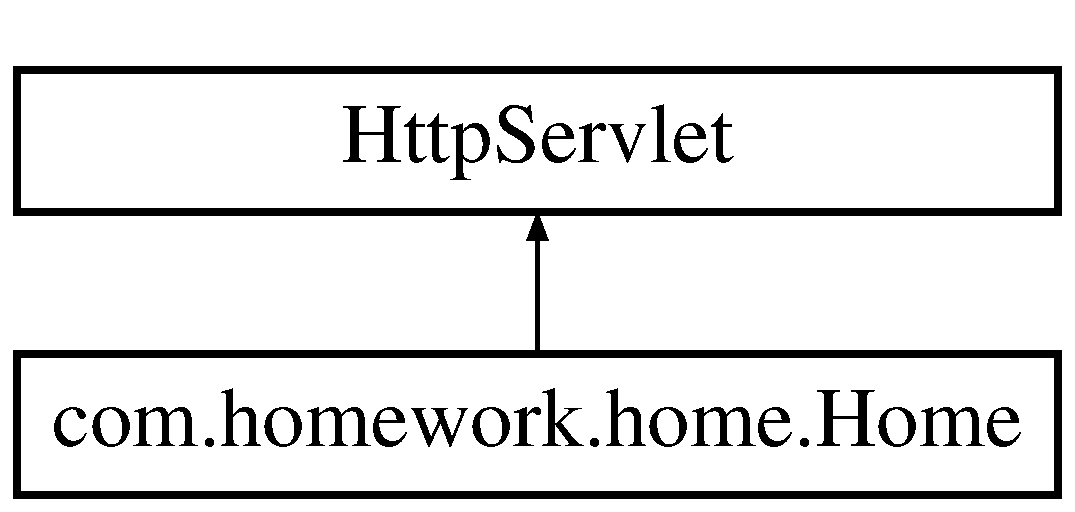
\includegraphics[height=2.000000cm]{classcom_1_1homework_1_1home_1_1_home}
\end{center}
\end{figure}
\subsection*{Public Member Functions}
\begin{DoxyCompactItemize}
\item 
\hyperlink{classcom_1_1homework_1_1home_1_1_home_ac5127b125cf55fbef4e84aaf0728fd72}{Home} ()
\end{DoxyCompactItemize}
\subsection*{Protected Member Functions}
\begin{DoxyCompactItemize}
\item 
void \hyperlink{classcom_1_1homework_1_1home_1_1_home_a390ad06ac932e0ab47bcad1469c9c174}{do\+Get} (Http\+Servlet\+Request request, Http\+Servlet\+Response response)  throws Servlet\+Exception, I\+O\+Exception 
\end{DoxyCompactItemize}
\subsection*{Static Private Attributes}
\begin{DoxyCompactItemize}
\item 
static final long \hyperlink{classcom_1_1homework_1_1home_1_1_home_ab7840589e7705ec054b07f9488dc9b4e}{serial\+Version\+U\+ID} = 1L
\end{DoxyCompactItemize}


\subsection{Constructor \& Destructor Documentation}
\index{com\+::homework\+::home\+::\+Home@{com\+::homework\+::home\+::\+Home}!Home@{Home}}
\index{Home@{Home}!com\+::homework\+::home\+::\+Home@{com\+::homework\+::home\+::\+Home}}
\subsubsection[{\texorpdfstring{Home()}{Home()}}]{\setlength{\rightskip}{0pt plus 5cm}com.\+homework.\+home.\+Home.\+Home (
\begin{DoxyParamCaption}
{}
\end{DoxyParamCaption}
)}\hypertarget{classcom_1_1homework_1_1home_1_1_home_ac5127b125cf55fbef4e84aaf0728fd72}{}\label{classcom_1_1homework_1_1home_1_1_home_ac5127b125cf55fbef4e84aaf0728fd72}


\subsection{Member Function Documentation}
\index{com\+::homework\+::home\+::\+Home@{com\+::homework\+::home\+::\+Home}!do\+Get@{do\+Get}}
\index{do\+Get@{do\+Get}!com\+::homework\+::home\+::\+Home@{com\+::homework\+::home\+::\+Home}}
\subsubsection[{\texorpdfstring{do\+Get(\+Http\+Servlet\+Request request, Http\+Servlet\+Response response)}{doGet(HttpServletRequest request, HttpServletResponse response)}}]{\setlength{\rightskip}{0pt plus 5cm}void com.\+homework.\+home.\+Home.\+do\+Get (
\begin{DoxyParamCaption}
\item[{Http\+Servlet\+Request}]{request, }
\item[{Http\+Servlet\+Response}]{response}
\end{DoxyParamCaption}
) throws Servlet\+Exception, I\+O\+Exception\hspace{0.3cm}{\ttfamily [protected]}}\hypertarget{classcom_1_1homework_1_1home_1_1_home_a390ad06ac932e0ab47bcad1469c9c174}{}\label{classcom_1_1homework_1_1home_1_1_home_a390ad06ac932e0ab47bcad1469c9c174}


\subsection{Member Data Documentation}
\index{com\+::homework\+::home\+::\+Home@{com\+::homework\+::home\+::\+Home}!serial\+Version\+U\+ID@{serial\+Version\+U\+ID}}
\index{serial\+Version\+U\+ID@{serial\+Version\+U\+ID}!com\+::homework\+::home\+::\+Home@{com\+::homework\+::home\+::\+Home}}
\subsubsection[{\texorpdfstring{serial\+Version\+U\+ID}{serialVersionUID}}]{\setlength{\rightskip}{0pt plus 5cm}final long com.\+homework.\+home.\+Home.\+serial\+Version\+U\+ID = 1L\hspace{0.3cm}{\ttfamily [static]}, {\ttfamily [private]}}\hypertarget{classcom_1_1homework_1_1home_1_1_home_ab7840589e7705ec054b07f9488dc9b4e}{}\label{classcom_1_1homework_1_1home_1_1_home_ab7840589e7705ec054b07f9488dc9b4e}


The documentation for this class was generated from the following file\+:\begin{DoxyCompactItemize}
\item 
src/com/homework/home/\hyperlink{_home_8java}{Home.\+java}\end{DoxyCompactItemize}

\hypertarget{classcom_1_1homework_1_1yunus_1_1_yunus}{}\section{com.\+homework.\+yunus.\+Yunus Class Reference}
\label{classcom_1_1homework_1_1yunus_1_1_yunus}\index{com.\+homework.\+yunus.\+Yunus@{com.\+homework.\+yunus.\+Yunus}}
Inheritance diagram for com.\+homework.\+yunus.\+Yunus\+:\begin{figure}[H]
\begin{center}
\leavevmode
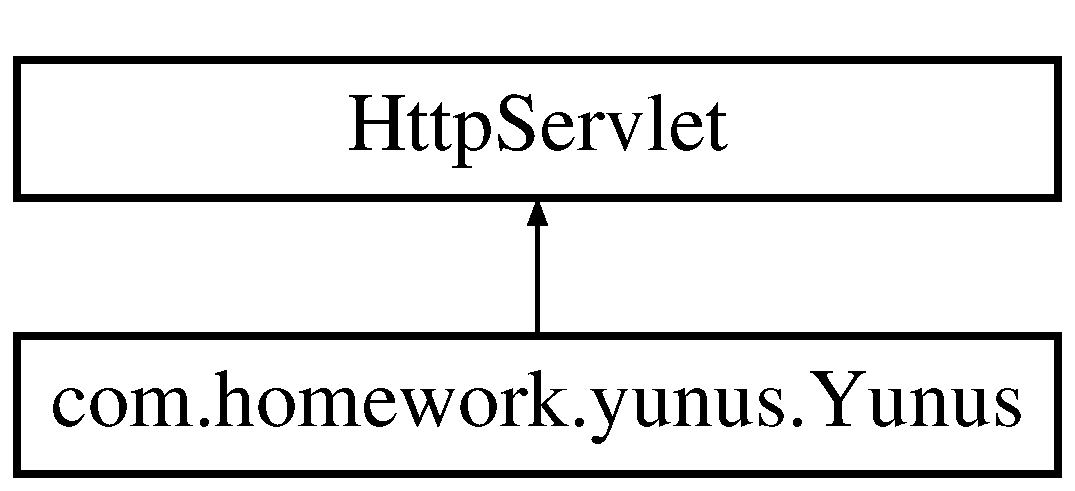
\includegraphics[height=2.000000cm]{classcom_1_1homework_1_1yunus_1_1_yunus}
\end{center}
\end{figure}
\subsection*{Public Member Functions}
\begin{DoxyCompactItemize}
\item 
\hyperlink{classcom_1_1homework_1_1yunus_1_1_yunus_a9d5871f9e874380b129c6dff31f1531b}{Yunus} ()
\end{DoxyCompactItemize}
\subsection*{Protected Member Functions}
\begin{DoxyCompactItemize}
\item 
void \hyperlink{classcom_1_1homework_1_1yunus_1_1_yunus_a2653e3f269da80881e2abfa6b30dc708}{do\+Get} (Http\+Servlet\+Request request, Http\+Servlet\+Response response)  throws Servlet\+Exception, I\+O\+Exception 
\item 
void \hyperlink{classcom_1_1homework_1_1yunus_1_1_yunus_abe7ecc6a6e297a44a50731348270ae17}{do\+Post} (Http\+Servlet\+Request req, Http\+Servlet\+Response resp)  throws Servlet\+Exception, I\+O\+Exception 
\end{DoxyCompactItemize}
\subsection*{Static Private Attributes}
\begin{DoxyCompactItemize}
\item 
static final long \hyperlink{classcom_1_1homework_1_1yunus_1_1_yunus_a135ed76b5ead6a58aa5f941be9477ed1}{serial\+Version\+U\+ID} = 1L
\end{DoxyCompactItemize}


\subsection{Detailed Description}
Servlet implementation of \hyperlink{classcom_1_1homework_1_1yunus_1_1_yunus}{Yunus}. \begin{DoxyAuthor}{Author}
\hyperlink{classcom_1_1homework_1_1yunus_1_1_yunus}{Yunus} 
\end{DoxyAuthor}


\subsection{Constructor \& Destructor Documentation}
\index{com\+::homework\+::yunus\+::\+Yunus@{com\+::homework\+::yunus\+::\+Yunus}!Yunus@{Yunus}}
\index{Yunus@{Yunus}!com\+::homework\+::yunus\+::\+Yunus@{com\+::homework\+::yunus\+::\+Yunus}}
\subsubsection[{\texorpdfstring{Yunus()}{Yunus()}}]{\setlength{\rightskip}{0pt plus 5cm}com.\+homework.\+yunus.\+Yunus.\+Yunus (
\begin{DoxyParamCaption}
{}
\end{DoxyParamCaption}
)}\hypertarget{classcom_1_1homework_1_1yunus_1_1_yunus_a9d5871f9e874380b129c6dff31f1531b}{}\label{classcom_1_1homework_1_1yunus_1_1_yunus_a9d5871f9e874380b129c6dff31f1531b}
\begin{DoxySeeAlso}{See also}
Http\+Servlet\+::\+Http\+Servlet() 
\end{DoxySeeAlso}


\subsection{Member Function Documentation}
\index{com\+::homework\+::yunus\+::\+Yunus@{com\+::homework\+::yunus\+::\+Yunus}!do\+Get@{do\+Get}}
\index{do\+Get@{do\+Get}!com\+::homework\+::yunus\+::\+Yunus@{com\+::homework\+::yunus\+::\+Yunus}}
\subsubsection[{\texorpdfstring{do\+Get(\+Http\+Servlet\+Request request, Http\+Servlet\+Response response)}{doGet(HttpServletRequest request, HttpServletResponse response)}}]{\setlength{\rightskip}{0pt plus 5cm}void com.\+homework.\+yunus.\+Yunus.\+do\+Get (
\begin{DoxyParamCaption}
\item[{Http\+Servlet\+Request}]{request, }
\item[{Http\+Servlet\+Response}]{response}
\end{DoxyParamCaption}
) throws Servlet\+Exception, I\+O\+Exception\hspace{0.3cm}{\ttfamily [protected]}}\hypertarget{classcom_1_1homework_1_1yunus_1_1_yunus_a2653e3f269da80881e2abfa6b30dc708}{}\label{classcom_1_1homework_1_1yunus_1_1_yunus_a2653e3f269da80881e2abfa6b30dc708}
Starting page of the application. \begin{DoxySeeAlso}{See also}
Http\+Servlet\+::do\+Get(\+Http\+Servlet\+Request request, Http\+Servlet\+Response response) 
\end{DoxySeeAlso}
$<$ Our writer to type html codes \index{com\+::homework\+::yunus\+::\+Yunus@{com\+::homework\+::yunus\+::\+Yunus}!do\+Post@{do\+Post}}
\index{do\+Post@{do\+Post}!com\+::homework\+::yunus\+::\+Yunus@{com\+::homework\+::yunus\+::\+Yunus}}
\subsubsection[{\texorpdfstring{do\+Post(\+Http\+Servlet\+Request req, Http\+Servlet\+Response resp)}{doPost(HttpServletRequest req, HttpServletResponse resp)}}]{\setlength{\rightskip}{0pt plus 5cm}void com.\+homework.\+yunus.\+Yunus.\+do\+Post (
\begin{DoxyParamCaption}
\item[{Http\+Servlet\+Request}]{req, }
\item[{Http\+Servlet\+Response}]{resp}
\end{DoxyParamCaption}
) throws Servlet\+Exception, I\+O\+Exception\hspace{0.3cm}{\ttfamily [protected]}}\hypertarget{classcom_1_1homework_1_1yunus_1_1_yunus_abe7ecc6a6e297a44a50731348270ae17}{}\label{classcom_1_1homework_1_1yunus_1_1_yunus_abe7ecc6a6e297a44a50731348270ae17}
Looks to the actions of the Servlet. Make methods work when buttons are pressed. $<$ Our writer to type html codes 

\subsection{Member Data Documentation}
\index{com\+::homework\+::yunus\+::\+Yunus@{com\+::homework\+::yunus\+::\+Yunus}!serial\+Version\+U\+ID@{serial\+Version\+U\+ID}}
\index{serial\+Version\+U\+ID@{serial\+Version\+U\+ID}!com\+::homework\+::yunus\+::\+Yunus@{com\+::homework\+::yunus\+::\+Yunus}}
\subsubsection[{\texorpdfstring{serial\+Version\+U\+ID}{serialVersionUID}}]{\setlength{\rightskip}{0pt plus 5cm}final long com.\+homework.\+yunus.\+Yunus.\+serial\+Version\+U\+ID = 1L\hspace{0.3cm}{\ttfamily [static]}, {\ttfamily [private]}}\hypertarget{classcom_1_1homework_1_1yunus_1_1_yunus_a135ed76b5ead6a58aa5f941be9477ed1}{}\label{classcom_1_1homework_1_1yunus_1_1_yunus_a135ed76b5ead6a58aa5f941be9477ed1}


The documentation for this class was generated from the following file\+:\begin{DoxyCompactItemize}
\item 
src/com/homework/yunus/\hyperlink{_yunus_8java}{Yunus.\+java}\end{DoxyCompactItemize}

\chapter{File Documentation}
\hypertarget{_home_8java}{}\section{src/com/homework/home/\+Home.java File Reference}
\label{_home_8java}\index{src/com/homework/home/\+Home.\+java@{src/com/homework/home/\+Home.\+java}}
\subsection*{Classes}
\begin{DoxyCompactItemize}
\item 
class \hyperlink{classcom_1_1homework_1_1home_1_1_home}{com.\+homework.\+home.\+Home}
\end{DoxyCompactItemize}
\subsection*{Packages}
\begin{DoxyCompactItemize}
\item 
package \hyperlink{namespacecom_1_1homework_1_1home}{com.\+homework.\+home}
\end{DoxyCompactItemize}

\hypertarget{_db_yunus_8java}{}\section{src/com/homework/yunus/\+Db\+Yunus.java File Reference}
\label{_db_yunus_8java}\index{src/com/homework/yunus/\+Db\+Yunus.\+java@{src/com/homework/yunus/\+Db\+Yunus.\+java}}
\subsection*{Classes}
\begin{DoxyCompactItemize}
\item 
class \hyperlink{classcom_1_1homework_1_1yunus_1_1_db_yunus}{com.\+homework.\+yunus.\+Db\+Yunus}
\end{DoxyCompactItemize}
\subsection*{Packages}
\begin{DoxyCompactItemize}
\item 
package \hyperlink{namespacecom_1_1homework_1_1yunus}{com.\+homework.\+yunus}
\end{DoxyCompactItemize}

\hypertarget{_yunus_8java}{}\section{src/com/homework/yunus/\+Yunus.java File Reference}
\label{_yunus_8java}\index{src/com/homework/yunus/\+Yunus.\+java@{src/com/homework/yunus/\+Yunus.\+java}}
\subsection*{Classes}
\begin{DoxyCompactItemize}
\item 
class \hyperlink{classcom_1_1homework_1_1yunus_1_1_yunus}{com.\+homework.\+yunus.\+Yunus}
\end{DoxyCompactItemize}
\subsection*{Packages}
\begin{DoxyCompactItemize}
\item 
package \hyperlink{namespacecom_1_1homework_1_1yunus}{com.\+homework.\+yunus}
\end{DoxyCompactItemize}

%--- End generated contents ---

% Index
\backmatter
\newpage
\phantomsection
\clearemptydoublepage
\addcontentsline{toc}{chapter}{Index}
\printindex

\end{document}
